\documentclass[manuscript]{acmart}

\setcopyright{none}
\citestyle{acmauthoryear}
\raggedbottom
\usepackage{tikz}

\acmConference[CI 2026]{ACM Collective Intelligence 2026}{September 27--30, 2026}{Virginia Tech Institute for Advanced Computing, near Washington, DC, USA}
\acmYear{2026}
\acmBooktitle{Proceedings of ACM Collective Intelligence 2026 (CI 2026)}

\begin{document}

\title{ODD+D Appendix for Comparing Legislative Mechanism Bundles}

\author{Anonymous Author(s)}
\renewcommand{\shortauthors}{Anonymous Author(s)}
\authorsaddresses{}

\begin{abstract}
This appendix documents the congressional institutional simulator using the ODD and ODD+D model-description conventions \citep{Grimm2010,Muller2013}. It describes entities, state variables, scheduling, adaptation, input data, submodels, outputs, empirical flow smoke tests, assumptions, and reproducibility commands for the simulator used in \emph{A Reproducible Simulation Framework for Comparing Legislative Mechanism Bundles}.
\end{abstract}

\begin{CCSXML}
<ccs2012>
<concept>
<concept_id>10010147.10010257</concept_id>
<concept_desc>Computing methodologies~Modeling and simulation</concept_desc>
<concept_significance>500</concept_significance>
</concept>
<concept>
<concept_id>10003120.10003121.10003124.10010392</concept_id>
<concept_desc>Human-centered computing~Collaborative and social computing theory, concepts and paradigms</concept_desc>
<concept_significance>300</concept_significance>
</concept>
</ccs2012>
\end{CCSXML}

\ccsdesc[500]{Computing methodologies~Modeling and simulation}
\ccsdesc[300]{Human-centered computing~Collaborative and social computing theory, concepts and paradigms}

\keywords{ODD+D, legislative simulation, institutional design, model documentation}

\maketitle

\section{Appendix Roadmap}

\begin{table}[!htbp]
  \caption{Where to look for common reviewer questions.}
  \label{tab:appendix-roadmap}
  \Description{A roadmap table mapping reviewer concerns to appendix tables and sections.}
  \small
  \begin{tabular}{p{0.43\linewidth}p{0.45\linewidth}}
    \toprule
    Reviewer concern & Where to look \\
    \midrule
    What assumptions generate the synthetic worlds? & Table~\ref{tab:appendix-formal-generator} and Section~\ref{sec:appendix-initialization} \\
    What is empirically checked? & Table~\ref{tab:empirical-validation-gap} and Section~\ref{sec:appendix-input-data} \\
    What weights enter the vote kernel? & Table~\ref{tab:appendix-vote-features} \\
    What are the selected main-campaign results? & Table~\ref{tab:scenario-averages}; full CSV in \texttt{reports/simulation-campaign-v21-paper.csv} \\
    What robustness probes exist? & Tables~\ref{tab:sensitivity-controls}, \ref{tab:pareto-front}, \ref{tab:mechanism-ablation-diagnostics}, and \ref{tab:manipulation-stress-diagnostics} \\
    What are the main limitations? & Section~\ref{sec:appendix-limitations} \\
    How is the artifact reproduced? & Section~\ref{sec:appendix-reproducibility} \\
    \bottomrule
  \end{tabular}
\end{table}

\section{Purpose}

The model compares legislative institutional designs under shared generated political worlds. Its purpose is to stress-test mechanisms that alter productivity, revision moderation, representative responsiveness, public-benefit alignment, minority protection, and resistance to capture. It is not a forecast of a specific Congress. It is a mechanism-comparison simulator: the same generated legislators and bills are routed through many institutional processes so differences can be attributed to procedural rules and incentive structures.

\section{Entities, State Variables, and Scales}

\subsection{Legislators}

Legislators have an identifier, party label, ideology, revision-moderation preference, party loyalty, constituency sensitivity, lobbying susceptibility, reputation sensitivity, district preference, district intensity, affected-group sensitivity, and a representation profile. The representation profile records chamber eligibility, represented population share, district magnitude, region label, elected/appointed mode, lower- and upper-house term lengths, renewal cohort, renewal cycle, next renewal round, and selector body. These values determine how the legislator weighs ideology, party pressure, constituent/public support, lobbying pressure, revision-moderation incentives, reputation, and concentrated harm before casting a final yes-or-no vote.

\subsection{Bills}

Bills have an identifier, title, proposer, proposer ideology, original and current policy position, public support, generated public benefit, public-benefit uncertainty, lobby pressure, private gain, salience, issue domain, anti-lobbying-reform flag, affected group, affected-group support, concentrated harm, compensation cost, cosponsor counts, amendment movement, lobbying channel spend, challenge status, citizen-review signals, active-law signals, and alternative-selection signals.

\subsection{Lobby Groups}

Lobby groups are explicit collective actors. Each group has an identifier, primary issue domain, issue-preference map, preferred policy position, budget, influence intensity, defensive multiplier, information bias, public-campaign skill, capture strategy, and public-support mismatch tolerance. Groups can spend through direct pressure, agenda-access pressure, information distortion, public campaigns, litigation or delay threats, and defensive anti-reform pressure.

\subsection{Institutional Processes}

An institutional process is a composable module. Processes can screen proposal access, apply leadership agenda control, modify public signals, spend lobbying or attention resources, route bills to procedural tracks, mediate amendments, evaluate affected-group harm, select among alternatives, conduct chamber votes, revise through conference committees, apply vetoes, apply judicial review, route through citizen initiatives or citizen agenda petitions, register enacted laws, or review laws later. The chamber-structure supplement adds chamber-specification, chamber-origin routing, second-chamber amendment and veto powers, last-offer bargaining, lower-house override, committee-assignment configuration, committee-role power, eligibility and retention filters, and ex ante review through insulated fiscal, electoral, audit, ethics, or legal-review bodies. The simulator also includes bounded linked modules for open floor calendars, discharge-petition committee bypass, district-population public signals, pairwise amendment tournaments, long-horizon proposer strategy, omnibus bargaining, campaign-finance influence systems, and constitutional-court architecture. The final decision still resolves to a yes-or-no outcome, enactment or rejection, and a post-bill status quo. Portfolio variants combine low-risk fast passage, middle-risk pairwise alternatives and mediation, high-risk citizen and harm review, proposal bonds, anti-capture safeguards, law-registry correction, and, in the expanded variant, public-opinion, influence-system, omnibus, and court-review proxies.

\section{Process Overview and Scheduling}

Each run follows a fixed schedule:

\begin{enumerate}
  \item Generate a world containing legislators, party positions, lobby groups, a status quo, and a bill stream.
  \item Build each scenario's legislative process from that world.
  \item For each bill, create a deterministic vote context containing party positions, status quo, and seeded randomness.
  \item Pass the bill through the scenario process chain.
  \item Record the bill outcome, including agenda disposition, vote totals, enactment, amendments, challenges, lobbying signals, public-review signals, and policy movement.
  \item Update the scenario's status quo when policy is enacted or rolled back.
  \item Aggregate outcomes into scenario metrics.
\end{enumerate}

Campaigns repeat this over many runs and assumption cases. Scenarios share generated worlds but use independent deterministic random streams, supporting paired comparison among institutions.

\section{Design Concepts}

\subsection{Basic Principles}

The model assumes legislative outcomes are shaped by proposal access, agenda scarcity, voting thresholds, committee and information structures, lobbying and capture, amendment opportunities, public review, concentrated harm, reversibility, and strategic actor adaptation.

\subsection{Emergence}

Productivity, revision moderation, capture, volatility, legitimacy, and gridlock emerge from bill-by-bill interactions. No actor directly optimizes the reported global metrics.

\subsection{Adaptation}

Proposers adapt over repeated bills. They can reduce proposal volume, delay timing, moderate risky bills, seek outside-bloc cosponsorship, reduce lobby exposure, add compensation amendments, lower risk tolerance after bad outcomes, and withdraw weak risky bills. Proposer state includes trust, proposal pace, risk tolerance, concession rate, lobby exposure, cooldown, and streak counters.

Lobby groups adapt over repeated bills. They track returns by channel, select capture strategies from learned returns and current bill conditions, change issue-specific spending multipliers, adjust overall budget intensity, increase reform-threat sensitivity when anti-lobbying bills become threatening, and maintain defensive pressure against reforms that would reduce lobbying influence.

Institutional state also adapts through proposal credits, proposal bonds, law registries, sunset review, challenge-token exhaustion, attention-token spending, norm erosion, judicial reversals, and active-law correction.

\subsection{Objectives}

Legislators vote according to weighted incentives. Proposers seek agenda access and enactment while learning to avoid reputational or procedural failure. Lobby groups seek policy movement toward their issue preferences and private gains while resisting anti-lobbying reforms. Institutions impose constraints and incentives whose tradeoffs are measured afterward.

\subsection{Learning and Prediction}

Learning is deterministic and bounded rather than a full reinforcement-learning procedure. Actors use local outcome signals: enactment, public support, public benefit, capture risk, concentrated harm, salience, private gain, prior failures, and prior channel returns.

\subsection{Stochasticity}

World generation, committee composition, citizen panels, bill signals, party-system profiles, and some routing decisions use seeded randomness. Identical seeds reproduce identical outputs.

\subsection{Observation}

The simulator reports productivity, floor load, enacted support, generated public benefit, cooperation, revision moderation, gridlock, access denial, committee rejection, challenge rate, chamber low-support passage, low-public-support enactment, policy shift, proposer gain, lobby capture, public alignment, anti-lobbying success, private-gain ratio, lobbying spend by channel, public benefit per lobby dollar, amendment rate, amendment movement, amendment overload, poison-pill rate, support gain after amendment, minority harm, concentrated-harm passage, compensation rate, legitimacy, enacted-policy quality, policy yield per submitted proposal, blockage reliance, public support, active-law welfare, implementation delay/capacity/failure risk, nonenforcement and underfunding risk, renewal pressure, reversal rate, correction delay, low-support active-law share, selected-alternative distance, proposer agenda advantage, alternative diversity, status-quo win rate, citizen-review metrics, citizen agenda petition metrics, open-calendar metrics, attention spending, objection-window use, public-will review, district alignment, cosponsorship, bond forfeiture, strategic decoys, proposer-access Gini, vetoes, overrides, chamber conflict, malapportionment, population-seat distortion, committee capture, eligibility exclusion, renewal staggering, recusal, ex ante review, review delay, and quiet-capture risk.
The main manuscript uses only the subset of metrics in its metric table; the full observation list is retained here to document implemented outputs for reproduction and future studies.

\section{Initialization}
\label{sec:appendix-initialization}

\texttt{WorldGenerator} creates legislators from party-system and ideology parameters, derives party positions, generates lobby groups by issue domain, chooses a scalar status quo, and generates bills around proposer ideal points. Generated values are bounded by implementation constraints and broad plausibility checks. Party-system profiles include ideological bins, two major parties with minor parties, fragmented multiparty systems, dominant-party systems, and weighted campaign profiles.

\begin{table*}
  \caption{Detailed generator variables and where they enter the model. This table expands the simplified assumptions table in the main paper.}
  \label{tab:appendix-formal-generator}
  \Description{A formal model table listing generated variables, distribution summaries, scenario tuning status, and model uses.}
  \scriptsize
  \resizebox{\textwidth}{!}{%
  \begin{tabular}{lllll}
    \toprule
    Component & Variable & Distribution or formula summary & Scenario tuned? & Main use \\
    \midrule
    Legislator ideal point & \(z_i\) & faction centers at \(\{-s,0,s\}\), \(s=0.25+0.65\rho\), Gaussian spread, clamp \([-1,1]\) & yes & vote kernel, parties \\
    Party and district signals & party, \(d_i\) & party bins or party-system profile; \(d_i=0.78z_i+N(0,0.18+0.10\rho)\) & yes & party pressure, district diagnostics \\
    Sensitivities & \(c_i,\pi_i,\kappa_i,\lambda_i,r_i\) & scenario center plus bounded Gaussian noise & yes & revision moderation, party, constituency, lobby, reputation weights \\
    Status quo & \(q_0\) & \(N(0,0.18)\), clamp \([-1,1]\); enacted bills update \(q_t\) & no & status-quo-relative voting \\
    Bill position & \(x_b\) & proposer-centered \(z_p+N(0,0.22)\), with adversarial shock variants & yes & vote kernel, policy shift \\
    Public support/benefit & \(p_b,g_b\) & \(g_b=0.34+0.34(1-|x_b|)-0.08 private+N(0,0.18)\); \(p_b=g_b+0.08\ell_b-0.05 private+N(0,0.22)\) & yes & support, yield, risk \\
    Lobby and private gain & \(\ell_b,private_b\) & \(\ell_b=N(0,L)\), \(private_b=0.72\max(0,\ell_b)+U(0,0.20)\), bounded & yes & access, capture, vote \\
    Harm and uncertainty & \(h_b,\sigma_b\) & harm rises with distance, salience, private gain, and noise; uncertainty rises with salience, signal mismatch, and lobbying & yes & harm thresholds, risk metrics \\
    \bottomrule
  \end{tabular}%
  }
\end{table*}

\section{Input Data and Empirical Flow Checks}
\label{sec:appendix-input-data}

Normal scenario runs use synthetic generated worlds. Empirical flow smoke tests read the tracked benchmark extract at \texttt{data/calibration/empirical-benchmarks.csv}. The extract maps empirical sources to simulator metrics and broad benchmark ranges. Named sources include Voteview roll-call data \citep{Voteview2021}, Congress.gov and govinfo bill histories \citep{CongressGovData,GovinfoBillStatus2020}, Comparative Agendas Project topic data \citep{ComparativeAgendasProject}, ParlGov party-system data \citep{ParlGov2024}, U.S. Lobbying Disclosure Act filings \citep{SenateLDA}, Center for Effective Lawmaking scores \citep{CenterEffectiveLawmaking,VoldenWiseman2014}, and V-Dem institutional indicators \citep{VDemDataset}.

The executable checker runs conventional scenarios and writes CSV and Markdown pass/fail reports under \texttt{reports/}. The pass is an empirical screen, not an automatic parameter fitter. Its benchmark ranges are intentionally broad and several are abstract proxies, so passing the screen should be read as minimum flow plausibility rather than validation. The empirical comparison checks include six documented samples: Congress.gov bill progression, Voteview roll calls, Senate LDA lobbying disclosures, and Congress.gov-derived topic, sponsor, and committee summaries. These samples support bill-attrition, floor-load, committee-report, coalition-size, party-unity, sponsor-concentration, topic-throughput, and lobbying-concentration checks. Optional API fixture samples are stored separately from raw empirical inputs; they test adapter shapes but are not used as validation evidence.

\begin{table}
\centering
\caption{Empirical boundary by source family. Held-out benchmark rows have a deterministic held-out empirical check; flow sanity and calibration proxy rows remain limited empirical screens; any synthetic-only row would lack usable raw inputs.}
\label{tab:empirical-validation-gap}
\small
\begin{tabular}{p{0.20\linewidth}p{0.20\linewidth}p{0.52\linewidth}}
\toprule
Source family & Status & Claim boundary / next source \\
\midrule
Congress.gov bill histories & held-out benchmark (available) & Supports held-out legislative-flow benchmarking only; does not validate public benefit or welfare Linkage: linked. Next: Replace bounded sample with full Congress.gov or govinfo bill census \\
govinfo bill and action records & calibration proxy (available) & Supports calibration ranges and source cross-checks; not full validation or a full bill census Linkage: metadata linked. Next: Expand the govinfo BILLSTATUS cross-check beyond the current bounded sample into a full bill/action census and review action-text differences before using it for stronger bill-flow claims. \\
Voteview roll-call data & held-out benchmark (available) & Supports held-out roll-call coalition benchmark and party-unity plausibility only; not district public opinion representation or public-support validation Linkage: metadata linked. Next: Expand roll-call-to-bill/action coverage beyond the current bounded crosswalk and join bill IDs to topics, district public opinion, sponsor histories, public laws, implementation, or court outcomes. \\
Comparative Agendas topic throughput & flow sanity check (available) & Supports agenda-flow plausibility; does not validate public value by topic Linkage: linked. Next: Map bills to CAP or another stable topic taxonomy \\
QoG and V-Dem comparative institutions & held-out benchmark (medium) & Supports held-out comparative bicameral-context plausibility and bounded simulator scenario-family metadata anchoring only; does not validate institutional fit bicameral disagreement or law-output productivity Linkage: metadata linked. Next: Add IPU/ParlGov chamber identifiers, observed country-year legislative-output rows, and bicameral disagreement data before making comparative institutional-fit or productivity claims. \\
Senate LDA lobbying disclosures & calibration proxy (available) & Supports spending observability and concentration only; not bill-level capture validation Linkage: partially linked. Next: Use the source-acquisition queue, external LDA mention review, and campaign-finance target-scope review to preserve committee/no-direct-committee source dispositions, acquire direct member target documents, independent contact and target sources, external campaign-finance source documents, and outcome-causality evidence while preserving the no-causal-capture boundary. \\
OpenFEC campaign finance & held-out benchmark (high) & Supports held-out campaign-finance concentration and outside-spending plausibility only; not bill-level influence or capture validation Linkage: partially linked. Next: Use the source-acquisition queue to preserve committee/no-direct-committee source dispositions and acquire direct member target documents, external campaign target/source documents, independent lobbying target/contact sources, and legislative outcomes and outcome-causality evidence before making any bill-specific campaign-finance influence claim. \\
Center for Effective Lawmaking and sponsor histories & held-out benchmark (available) & Supports held-out sponsor proposal-access concentration benchmarking and bounded sponsor-to-bill metadata linkage only; not full member effectiveness or sponsor-success validation Linkage: metadata linked. Next: Replace the bounded sponsor aggregate with complete sponsor histories or licensed CEL-style effectiveness data, and connect sponsor bills to roll calls, committees, issues, district opinion, finance, lobbying, and outcomes. \\
District public opinion and affected groups & held-out benchmark (high) & Supports held-out district survey aggregation and one bounded source-reviewed historical related-issue pilot with two privacy-thresholded annual direct-weighted district estimates; not exact or contemporaneous bill support MRP design-based uncertainty validated boundary equivalence bill-text-specific affected-group mapping causal representation public benefit or model validation Linkage: partially linked. Next: Use the source packets, survey-source crosswalk, ACS district-context, proxy review, candidate-item review, response-code distribution review, codebook review, official bill text, and retained historical related-issue estimates as the bounded frame; then add exact or closer contemporaneous bill-topic questions, design-based uncertainty or MRP where needed, and bill-text-specific affected-population, support, and harm evidence. \\
Committee hearing markup referral and discharge records & flow sanity check (available) & Supports rough committee reporting only; hearings markups and amendments remain thin Linkage: linked. Next: Add committee hearing calendars markups amendments and discharge petitions \\
Court review and invalidation & held-out benchmark (medium) & Supports held-out merits-case court-review plausibility and bounded U.S.C.-section authority-overlap metadata only; emergency-order behavior and direct case-to-public-law review remain unvalidated Linkage: partially linked. Next: Add direct case-to-statute/public-law identifiers, lower-court or emergency-order coding, and reviewed links from challenged laws to bill and implementation records. \\
Rulemaking implementation and enforcement & held-out benchmark (high) & Supports held-out final-rule implementation-delay plausibility only; complete comment records, enforcement, nonenforcement, and underfunding remain unvalidated Linkage: metadata linked. Next: Add higher-volume Regulations.gov comment-record retrieval, broader sanitized comment-detail sampling with explicit partial-coverage flags, attachment review where needed, Unified Agenda stages, agency enforcement rows, appropriations capacity, and reviewed statute-to-rule coverage beyond bounded authority and proposed-history metadata. \\
Statutory revision and law lineage & held-out benchmark (high) & Supports held-out statutory revision-activity plausibility bounded official OLRC public-law marker review target review packets and a thirteen-public-law source-reviewed target-section diff pilot only; not full target-statute longitudinal lineage observed expiration outcomes effective statutory text or direct court invalidation Linkage: metadata linked. Next: Use the target-reference resolution candidate report to confirm that no ambiguous packet blockers currently require bounded concrete U.S.C. candidate confirmation and 0 unresolved ambiguous packet blockers remain, then use the target-packet source-gap queue and source-gap disposition review to resolve current OLRC pages without public-law markers, build downstream packets for current pages with public-law markers, and expand source-reviewed no-packet dispositions for current-scan source-gap rows before treating queued rows as packet-ready; then use the target-packet expansion queue and complete-lineage expansion queue to expand the U.S.C. target inventory from source-scan candidates, audit related subsections, notes, amendments, repeals, redesignations, and cross-references, source-review any post-enactment raw SCDB target-section overlaps, and add higher-volume comment-record retrieval, broader sanitized comment-detail sampling with explicit partial-coverage flags, enforcement records, appropriations capacity, and direct court-review identifiers. \\
\bottomrule
\end{tabular}
\end{table}


\section{Submodels}

\subsection{Voting}

Legislators cast \texttt{YAY} or \texttt{NAY} through weighted influences: ideology, party, constituency/public support, lobbying, revision-moderation preference, reputation, and affected-group sensitivity.

\begin{table*}
  \caption{Vote-score feature functions and weights. The anti-capture kernel changes weights; affected-group variables enter procedural thresholds and metrics rather than the base yes/no vote score.}
  \label{tab:appendix-vote-features}
  \Description{A table listing vote-score feature functions and their standard and anti-capture weights.}
  \scriptsize
  \resizebox{\textwidth}{!}{%
  \begin{tabular}{llll}
    \toprule
    Feature & Function summary & Standard \(w_k\) & Anti-capture \(w_k\) \\
    \midrule
    Ideology & \((u_i(x_b)-u_i(q_t))(0.75+salience_b)\) & 1.45 & 1.45 \\
    Party & party loyalty times \(u_{party}(x_b)-u_{party}(q_t)\) & 0.85 & 0.78 \\
    Constituency/public & constituency sensitivity times \(2(p_b-0.5)\) & 0.95 & 1.12 \\
    Lobbying & lobby sensitivity times \(\ell_b\) & 0.55 & 0.14 \\
    Revision moderation & revision-moderation preference times \(0.45\) moderation \(+0.35\) public legitimacy \(+0.20\) incrementalism & 0.75 & 0.82 \\
    Reputation & reputation sensitivity times unpopular-bill and lobby-capture penalties & 0.55 & 0.92 \\
    Noise & seeded Gaussian perturbation before logistic voting & sd 0.25 & sd 0.25 \\
    \bottomrule
  \end{tabular}%
  }
\end{table*}

\subsection{Proposal Access and Agenda Scarcity}

Access rules include open access, open floor calendars with abusive-access screens, citizen agenda petitions, viability screens, scalar proposal costs, public-value waivers, lobby surcharges, member quotas, leadership agenda control, public-interest screens, anti-capture proposal-access screens, cross-bloc cosponsorship gates, affected-group sponsor gates, proposal bonds, earned proposal credits, agenda lotteries, and quadratic attention budgets.

\subsection{Committees and Information}

Committee gatekeeping can reject proposals before floor consideration. Committee information processes move public-signal estimates toward generated public benefit with composition-dependent accuracy. Configured committee selection can vary issue domain, random seed, party quota, proportional assignment, expertise weighting, independence weighting, leadership control, rotation memory, chair allocation, quorum party balance, citizen advisory weight, and topic-referral authority. Committee-power processes distinguish priority queues, veto players, fast-track certification, scrutiny and audit, public accounts, legal/drafting review, and discharge-petition targets.

\subsection{Chamber Structure, Eligibility, and Independent Review}

Chamber specifications define equal-population, proportional, mixed-member, territorial, malapportioned, appointed, indirect, functional, or mixed elected/appointed chambers. Bicameral routing variants can change origination, emergency routing, second-chamber preclearance, amendment-only powers, absolute or territorial vetoes, suspensive vetoes, navette, mediation, last-offer bargaining, joint sittings, and lower-house overrides. Eligibility and retention filters model stylized age, residency, language, expertise, conflict, attendance, capture-risk, dual-office, party/executive overlap, recusal, cooling-off, term-limit, recall, public-support retention, and sanctions rules. Ex ante review variants model optional referral, mandatory high-risk review, advisory opinions, suspensive objections, mandatory clearance, qualified override, and deadline-limited review by insulated fiscal, electoral, audit, ethics, cost-estimator, regulator, or boundary institutions.

\subsection{Challenge and Objection}

Challenge vouchers allocate scarce blocking rights to parties or members. Q-member escalation lets a sufficient number of legislators trigger active review. Public objection windows route contested bills to active voting, higher thresholds, or repeal review depending on scenario.

\subsection{Lobbying}

Budgeted lobbying modifies bill pressure and public signals through channel-specific spending. Anti-capture variants include transparency, public financing, public advocates, blind review, audits, sanctions, and defensive-spend caps. Adaptive lobbying learns from channel returns and reform threats.

\subsection{Amendment and Mediation}

Structured mediation moves risky proposals toward weighted institutional targets. Multi-round mediation models repeated amendments, costs, concession limits, poison-pill risk, capacity pressure, public-support improvement against a no-amendment counterfactual, proposer-advantage reduction, and compensation for concentrated harm.

\subsection{Distributional Harm}

Harm-weighted thresholds, compensation amendments, and affected-group consent mechanisms distinguish broad aggregate benefit from concentrated minority loss.

\subsection{Citizen Mini-Publics}

Citizen panels simulate sampling noise, information quality, manipulation risk, informed support, benefit estimates, and legitimacy. Panel output can affect burden-shifting eligibility, active-vote routing, final threshold, agenda priority, or affirmative majority burden of proof. Citizen agenda-petition paths separate raw support from costly participation signals, public-support intensity, and cheap signal distortion caused by organized amplification.

\subsection{Leadership, Direct Democracy, and Judicial Review}

Leadership agenda control schedules bills using observable public support, salience, uncertainty, majority-party fit, capture risk, and concentrated-harm risk rather than generated true welfare. Citizen-initiative processes let sufficiently salient, high-support proposals bypass legislative floor blockage through a public referendum. Conference-committee processes revise near-miss bicameral bills toward a bargaining target before chamber revotes. Judicial-review processes can invalidate enacted laws with high rights-like harm, uncertainty, policy shock, or capture risk.

\subsection{Alternatives, Package Bargaining, Norm Erosion, and Law Registry}

Competing-alternative processes generate same-domain alternatives and select by public benefit, public support, chamber-median proximity, or pairwise majority before final ratification. Pairwise amendment tournaments use the same selector logic for amended versions, making amendment control an explicit pre-ratification stage rather than only a final yes/no vote. Package-bargaining processes approximate revision through side-payment costs, implementation-delay costs, modest policy movement, and harm-reducing package trades. Norm-erosion processes raise procedural delay and reduce public support signals under high contention. Law-registry processes allow enacted laws to persist, face implementation delay, operate under capacity/nonenforcement/underfunding risk, be renewed under lobbying pressure, and be repealed or partially rolled back after review.

\section{Experimental Design}

The main submitted evidence comes from the main comparison campaign. That campaign joins broad assumption cases, adversarial proposal-generator cases, party-system sensitivity cases, and a stylized rising-contention timeline in one artifact. The main manuscript focuses on the stylized U.S.-like benchmark, simple majority, committee regular order, discharge petition, open floor calendar, a combined content-selection family, anti-capture access, harm-weighted majority, a small burden-shifting stress-test family, and a portfolio hybrid. The appendix tables report separate pairwise-alternative and amendment-tournament rows plus the broader implemented catalog, including leadership agenda control, chamber and committee variants, citizen petitions and initiatives, mini-publics, agenda scarcity, package bargaining, review and correction systems, adaptive routing, norm erosion, and influence-system safeguards. Adversarial generator cases test high-benefit extreme reform, popular harmful bills, moderate capture, delayed-benefit reform, concentrated rights-like harm, anti-lobbying backlash, revision dilution, useful lobbying information, and public-opinion error. Follow-up diagnostics include mechanism ablations, manipulation-stress campaigns, chamber-structure family/stress screens, and empirical flow smoke tests that map optional raw empirical summaries to simulator proxy metrics.

% Auto-generated by paper/scripts/generate_figures.py
\begin{table*}
  \caption{Selected core metrics from the main campaign, grouped by mechanism family. Entries are median [IQR] across broad and adversarial cases; the appendix reports mean/range, yield, seed diagnostics, and separate PAIR/AMT rows.}
  \label{tab:scenario-averages}
  \Description{A generated compact table comparing representative institutional families from the main comparison campaign.}
  \scriptsize
  \setlength{\fboxsep}{0.8pt}
  \resizebox{\textwidth}{!}{%
  \begin{tabular}{llrrrrrrr}
    \toprule
    Label & Representative system & Prod. $\uparrow$ & Rev. mod. $\uparrow$ & Public $\uparrow$ & Low supp. $\downarrow$ & Risk ctrl. $\uparrow$ & Admin feas. $\uparrow$ & Example profile $\uparrow$ \\
    \midrule
    \textbf{CUR*} & \textbf{Stylized U.S.-like benchmark} & \colorbox{black!7}{\makebox[17.5mm][c]{\strut \textbf{0.05 [0.03,0.06]}}} & \colorbox{black!17}{\makebox[17.5mm][c]{\strut \textbf{0.37 [0.36,0.38]}}} & \colorbox{black!30}{\makebox[17.5mm][c]{\strut \textbf{0.79 [0.78,0.80]}}} & \colorbox{black!37}{\makebox[17.5mm][c]{\strut \textbf{0.01 [0.00,0.01]}}} & \colorbox{black!35}{\makebox[17.5mm][c]{\strut \textbf{0.94 [0.92,0.94]}}} & \colorbox{black!36}{\makebox[17.5mm][c]{\strut \textbf{0.02 [0.01,0.02]}}} & \colorbox{black!23}{\makebox[17.5mm][c]{\strut \textbf{0.57 [0.56,0.58]}}} \\
    SM & Simple majority & \colorbox{black!14}{\makebox[17.5mm][c]{\strut 0.27 [0.22,0.32]}} & \colorbox{black!12}{\makebox[17.5mm][c]{\strut 0.23 [0.23,0.25]}} & \colorbox{black!27}{\makebox[17.5mm][c]{\strut 0.69 [0.67,0.70]}} & \colorbox{black!31}{\makebox[17.5mm][c]{\strut 0.19 [0.18,0.23]}} & \colorbox{black!33}{\makebox[17.5mm][c]{\strut 0.87 [0.85,0.88]}} & \colorbox{black!35}{\makebox[17.5mm][c]{\strut 0.07 [0.07,0.07]}} & \colorbox{black!22}{\makebox[17.5mm][c]{\strut 0.54 [0.53,0.55]}} \\
    COMM & Committee regular order & \colorbox{black!10}{\makebox[17.5mm][c]{\strut 0.16 [0.13,0.19]}} & \colorbox{black!14}{\makebox[17.5mm][c]{\strut 0.29 [0.28,0.29]}} & \colorbox{black!29}{\makebox[17.5mm][c]{\strut 0.74 [0.73,0.74]}} & \colorbox{black!34}{\makebox[17.5mm][c]{\strut 0.09 [0.07,0.10]}} & \colorbox{black!34}{\makebox[17.5mm][c]{\strut 0.91 [0.88,0.92]}} & \colorbox{black!36}{\makebox[17.5mm][c]{\strut 0.03 [0.03,0.03]}} & \colorbox{black!23}{\makebox[17.5mm][c]{\strut 0.55 [0.54,0.56]}} \\
    DIS & Discharge petition & \colorbox{black!10}{\makebox[17.5mm][c]{\strut 0.14 [0.09,0.17]}} & \colorbox{black!15}{\makebox[17.5mm][c]{\strut 0.31 [0.30,0.31]}} & \colorbox{black!29}{\makebox[17.5mm][c]{\strut 0.76 [0.74,0.76]}} & \colorbox{black!36}{\makebox[17.5mm][c]{\strut 0.04 [0.03,0.04]}} & \colorbox{black!35}{\makebox[17.5mm][c]{\strut 0.93 [0.92,0.94]}} & \colorbox{black!35}{\makebox[17.5mm][c]{\strut 0.08 [0.07,0.08]}} & \colorbox{black!23}{\makebox[17.5mm][c]{\strut 0.56 [0.55,0.56]}} \\
    OPEN & Open floor calendar & \colorbox{black!15}{\makebox[17.5mm][c]{\strut 0.31 [0.25,0.37]}} & \colorbox{black!13}{\makebox[17.5mm][c]{\strut 0.24 [0.23,0.26]}} & \colorbox{black!26}{\makebox[17.5mm][c]{\strut 0.67 [0.67,0.68]}} & \colorbox{black!29}{\makebox[17.5mm][c]{\strut 0.25 [0.22,0.26]}} & \colorbox{black!32}{\makebox[17.5mm][c]{\strut 0.85 [0.84,0.86]}} & \colorbox{black!34}{\makebox[17.5mm][c]{\strut 0.10 [0.09,0.10]}} & \colorbox{black!22}{\makebox[17.5mm][c]{\strut 0.54 [0.53,0.56]}} \\
    SEL & Content-selection family & \colorbox{black!22}{\makebox[17.5mm][c]{\strut 0.54 [0.49,0.56]}} & \colorbox{black!21}{\makebox[17.5mm][c]{\strut 0.50 [0.48,0.52]}} & \colorbox{black!30}{\makebox[17.5mm][c]{\strut 0.79 [0.77,0.79]}} & \colorbox{black!37}{\makebox[17.5mm][c]{\strut 0.00 [0.00,0.00]}} & \colorbox{black!35}{\makebox[17.5mm][c]{\strut 0.94 [0.93,0.95]}} & \colorbox{black!28}{\makebox[17.5mm][c]{\strut 0.28 [0.28,0.29]}} & \colorbox{black!27}{\makebox[17.5mm][c]{\strut 0.67 [0.66,0.69]}} \\
    ACG & Anti-capture access & \colorbox{black!13}{\makebox[17.5mm][c]{\strut 0.26 [0.20,0.30]}} & \colorbox{black!13}{\makebox[17.5mm][c]{\strut 0.24 [0.23,0.25]}} & \colorbox{black!28}{\makebox[17.5mm][c]{\strut 0.71 [0.68,0.71]}} & \colorbox{black!32}{\makebox[17.5mm][c]{\strut 0.16 [0.15,0.20]}} & \colorbox{black!34}{\makebox[17.5mm][c]{\strut 0.89 [0.88,0.90]}} & \colorbox{black!35}{\makebox[17.5mm][c]{\strut 0.06 [0.06,0.07]}} & \colorbox{black!23}{\makebox[17.5mm][c]{\strut 0.55 [0.54,0.56]}} \\
    HARM & Harm-weighted majority & \colorbox{black!13}{\makebox[17.5mm][c]{\strut 0.25 [0.18,0.27]}} & \colorbox{black!13}{\makebox[17.5mm][c]{\strut 0.24 [0.23,0.27]}} & \colorbox{black!27}{\makebox[17.5mm][c]{\strut 0.70 [0.68,0.70]}} & \colorbox{black!31}{\makebox[17.5mm][c]{\strut 0.19 [0.18,0.23]}} & \colorbox{black!33}{\makebox[17.5mm][c]{\strut 0.89 [0.87,0.89]}} & \colorbox{black!35}{\makebox[17.5mm][c]{\strut 0.07 [0.07,0.07]}} & \colorbox{black!22}{\makebox[17.5mm][c]{\strut 0.54 [0.53,0.55]}} \\
    DP & Burden-shifting stress case & \colorbox{black!32}{\makebox[17.5mm][c]{\strut 0.84 [0.84,0.89]}} & \colorbox{black!8}{\makebox[17.5mm][c]{\strut 0.11 [0.10,0.13]}} & \colorbox{black!23}{\makebox[17.5mm][c]{\strut 0.56 [0.54,0.57]}} & \colorbox{black!21}{\makebox[17.5mm][c]{\strut 0.50 [0.47,0.52]}} & \colorbox{black!25}{\makebox[17.5mm][c]{\strut 0.62 [0.61,0.63]}} & \colorbox{black!35}{\makebox[17.5mm][c]{\strut 0.07 [0.07,0.07]}} & \colorbox{black!23}{\makebox[17.5mm][c]{\strut 0.55 [0.54,0.56]}} \\
    DPM & Burden shift + mediation & \colorbox{black!31}{\makebox[17.5mm][c]{\strut 0.81 [0.72,0.89]}} & \colorbox{black!12}{\makebox[17.5mm][c]{\strut 0.22 [0.21,0.26]}} & \colorbox{black!24}{\makebox[17.5mm][c]{\strut 0.61 [0.59,0.64]}} & \colorbox{black!24}{\makebox[17.5mm][c]{\strut 0.40 [0.34,0.43]}} & \colorbox{black!29}{\makebox[17.5mm][c]{\strut 0.74 [0.70,0.75]}} & \colorbox{black!30}{\makebox[17.5mm][c]{\strut 0.21 [0.19,0.22]}} & \colorbox{black!24}{\makebox[17.5mm][c]{\strut 0.58 [0.57,0.60]}} \\
    PORT & Portfolio hybrid & \colorbox{black!21}{\makebox[17.5mm][c]{\strut 0.51 [0.44,0.58]}} & \colorbox{black!18}{\makebox[17.5mm][c]{\strut 0.41 [0.40,0.45]}} & \colorbox{black!29}{\makebox[17.5mm][c]{\strut 0.76 [0.76,0.78]}} & \colorbox{black!36}{\makebox[17.5mm][c]{\strut 0.03 [0.01,0.04]}} & \colorbox{black!35}{\makebox[17.5mm][c]{\strut 0.93 [0.93,0.93]}} & \colorbox{black!30}{\makebox[17.5mm][c]{\strut 0.23 [0.23,0.24]}} & \colorbox{black!25}{\makebox[17.5mm][c]{\strut 0.64 [0.63,0.66]}} \\
    \bottomrule
  \end{tabular}%
  }
  \par\smallskip\footnotesize \emph{Note:} Example profile is one revision-moderation-weighted sensitivity check: $0.30\,\mathrm{Rev.\ mod.}+0.20\,\mathrm{Prod.}+0.20\,\mathrm{Risk\ ctrl.}+0.15\,\mathrm{Admin\ feas.}+0.15\,\mathrm{Public}$. Admin feas. is the inverse of the administrative-cost index shown in the Admin column. Low supp. is low-public-support enactment. The asterisk marks the stylized U.S.-like conventional benchmark. Cell values carry the comparison; shading follows the column arrow as a secondary cue.
\end{table*}


The dense full scenario-average table is not repeated in the PDF appendix. Full numeric outputs, including separate pairwise-alternative and amendment-tournament rows, are provided in \texttt{reports/simulation-campaign-v21-paper.csv}; the generated LaTeX full table remains in \texttt{paper/figures/scenario\_averages\_full\_table.tex} for local inspection.

The following sensitivity and fairness probes are not validation evidence. They test whether the framework exposes dependence on generator assumptions and whether major qualitative patterns survive limited alternative worlds.

% Auto-generated by paper/scripts/generate_figures.py
\begin{table*}
  \caption{Appendix generator-sensitivity and fairness-control details. These rows summarize robustness probes; they are not validation evidence.}
  \label{tab:sensitivity-controls}
  \Description{A generated table summarizing generator sensitivity cases and fairness-control comparisons.}
  \scriptsize
  \setlength{\tabcolsep}{2.0pt}
  \resizebox{\textwidth}{!}{%
  \begin{tabular}{llll}
    \toprule
    Type & Check & Result & Interpretation \\
    \midrule
    Generator & Extreme-beneficial reform & top PORT 0.72; SEL 0.69; DPM 0.58; DP low supp. 0.57 & Tests whether high-distance proposals can carry high generated public benefit. \\
    Generator & Revision dilution & top PORT 0.71; SEL 0.67; DPM 0.57; DP low supp. 0.67 & Tests whether moderation can reduce generated public benefit. \\
    Generator & Lobby information & top SEL 0.74; PORT 0.71; DPM 0.65; DP low supp. 0.28 & Tests useful organized information rather than only capture pressure. \\
    Generator & Public-opinion error & top PORT 0.68; SEL 0.68; DPM 0.62; DP low supp. 0.41 & Tests noisy or systematically biased public-support signals. \\
    Generator & Minority-rights harm & top SEL 0.66; PORT 0.64; DPM 0.63; DP low supp. 0.19 & Tests majority support paired with concentrated rights-like harm. \\
    Generator & Technocratic delay & top PORT 0.69; SEL 0.66; DPM 0.61; DP low supp. 0.75 & Tests low initial support with delayed generated public benefit. \\
    Fairness & Conventional revision & CUR P 0.05, M 0.36, R 0.93, A 0.02; PROC P 0.05, M 0.32, R 0.93, A 0.03 & Gives the conventional family conference/review content improvement. \\
    Fairness & Majority mediation & SM P 0.33, M 0.24, R 0.85, A 0.07; SMED P 0.40, M 0.22, R 0.80, A 0.19 & Compares simple majority with a mediation content-improvement step. \\
    Fairness & Committee amendment & COMM P 0.21, M 0.28, R 0.89, A 0.03; CAMD P 0.12, M 0.32, R 0.93, A 0.07 & Compares committee gatekeeping with committee information/amendment power. \\
    \bottomrule
  \end{tabular}%
  }
  \par\smallskip\footnotesize \emph{Note:} P is productivity, M is revision moderation, R is risk control, and A is administrative cost. Fairness rows compare content-improvement variants; they do not impose a hard cost-constrained reoptimization.
\end{table*}

% Auto-generated by paper/scripts/generate_figures.py
\begin{table*}
  \centering
  \begin{minipage}[t]{0.39\textwidth}
    \centering
    \caption{Pareto-front scenarios under productivity, compromise, and risk control.}
    \label{tab:pareto-front}
    \scriptsize
    \setlength{\tabcolsep}{2.2pt}
    \resizebox{\linewidth}{!}{%
  \begin{tabular}{llrrrrr}
    \toprule
    Label & Role & Prod. $\uparrow$ & Comp. $\uparrow$ & Risk $\uparrow$ & Weak mand. $\downarrow$ & Admin $\downarrow$ \\
    \midrule
    DP & Throughput endpoint & 0.866 & 0.136 & 0.629 & 0.472 & 0.070 \\
    DPM & Throughput with mediation/challenge & 0.802 & 0.243 & 0.723 & 0.374 & 0.206 \\
    XPORT & Non-dominated profile & 0.783 & 0.463 & 0.904 & 0.003 & 0.586 \\
    PAIR & Alternative-comparison endpoint & 0.542 & 0.502 & 0.937 & 0.002 & 0.285 \\
    AMT & Non-dominated profile & 0.537 & 0.502 & 0.937 & 0.002 & 0.284 \\
    \bottomrule
  \end{tabular}
    }
    \par\smallskip\scriptsize \emph{Note:} The frontier changes if administrative feasibility, welfare, or rights/harm priorities are hard objectives.
  \end{minipage}\hfill
  \begin{minipage}[t]{0.58\textwidth}
    \centering
    % Auto-generated by scripts/reporting/write_paper_diagnostics.py
\begin{table*}
  \caption{Ablation diagnostics for selected mechanisms.}
  \label{tab:mechanism-ablation-diagnostics}
  \scriptsize
  \setlength{\tabcolsep}{2.2pt}
  \resizebox{\linewidth}{!}{%
  \begin{tabular}{llrrrr}
    \toprule
    Mechanism & Removed or replaced component & Directional & Rev. mod. & Low supp. reduction & Admin added \\
    \midrule
    Policy tournament & No alternatives & +0.056 & +0.266 & +0.217 & +0.219 \\
    Risk routing & No jury lane & -0.002 & +0.000 & +0.001 & +0.008 \\
    Anti-capture & Screen only & +0.024 & +0.000 & +0.043 & +0.005 \\
    Package bargaining & Scalar package & -0.015 & -0.002 & +0.004 & +0.065 \\
    Reversibility & No registry & -0.009 & -0.009 & -0.034 & +0.044 \\
    \bottomrule
  \end{tabular}
  }
  \par\smallskip\scriptsize \emph{Note:} Positive values indicate how much the original mechanism improved relative to the ablated variant, except Admin added, where positive means additional procedural cost in the original mechanism.
\end{table*}

\begin{table*}
  \caption{Manipulation-stress losses for selected mechanisms.}
  \label{tab:manipulation-stress-diagnostics}
  \scriptsize
  \setlength{\tabcolsep}{2.2pt}
  \resizebox{\linewidth}{!}{%
  \begin{tabular}{llrrrr}
    \toprule
    Stress case & Attack or perturbation & Directional loss & Rev. mod. loss & Low supp. added & Admin added \\
    \midrule
    Tournament attack & Clones/decoys & +0.087 & +0.046 & +0.010 & -0.077 \\
    Citizen-panel manipulation & Noisy panel & -0.002 & +0.018 & -0.005 & +0.000 \\
    Bad-faith harm claims & Loose claims & -0.002 & -0.018 & -0.018 & +0.000 \\
    Objection astroturf & Astroturf/noise & +0.012 & -0.006 & +0.003 & +0.010 \\
    Agenda flooding & Proposal flood & +0.008 & -0.011 & +0.007 & -0.001 \\
    \bottomrule
  \end{tabular}
  }
  \par\smallskip\scriptsize \emph{Note:} Positive values are losses or added burden under bounded manipulation stress. Low supp. is low-public-support enactment.
\end{table*}

  \end{minipage}
  \Description{Two generated side-by-side tables. The first lists Pareto-front scenarios under productivity, compromise, and risk control; the second lists selected mechanism ablations and manipulation stress tests.}
\end{table*}

% Auto-generated by scripts/reporting/write_paper_diagnostics.py
\begin{table*}
  \caption{Ablation diagnostics for selected mechanisms.}
  \label{tab:mechanism-ablation-diagnostics}
  \scriptsize
  \setlength{\tabcolsep}{2.2pt}
  \resizebox{\linewidth}{!}{%
  \begin{tabular}{llrrrr}
    \toprule
    Mechanism & Removed or replaced component & Directional & Rev. mod. & Low supp. reduction & Admin added \\
    \midrule
    Policy tournament & No alternatives & +0.056 & +0.266 & +0.217 & +0.219 \\
    Risk routing & No jury lane & -0.002 & +0.000 & +0.001 & +0.008 \\
    Anti-capture & Screen only & +0.024 & +0.000 & +0.043 & +0.005 \\
    Package bargaining & Scalar package & -0.015 & -0.002 & +0.004 & +0.065 \\
    Reversibility & No registry & -0.009 & -0.009 & -0.034 & +0.044 \\
    \bottomrule
  \end{tabular}
  }
  \par\smallskip\scriptsize \emph{Note:} Positive values indicate how much the original mechanism improved relative to the ablated variant, except Admin added, where positive means additional procedural cost in the original mechanism.
\end{table*}

\begin{table*}
  \caption{Manipulation-stress losses for selected mechanisms.}
  \label{tab:manipulation-stress-diagnostics}
  \scriptsize
  \setlength{\tabcolsep}{2.2pt}
  \resizebox{\linewidth}{!}{%
  \begin{tabular}{llrrrr}
    \toprule
    Stress case & Attack or perturbation & Directional loss & Rev. mod. loss & Low supp. added & Admin added \\
    \midrule
    Tournament attack & Clones/decoys & +0.087 & +0.046 & +0.010 & -0.077 \\
    Citizen-panel manipulation & Noisy panel & -0.002 & +0.018 & -0.005 & +0.000 \\
    Bad-faith harm claims & Loose claims & -0.002 & -0.018 & -0.018 & +0.000 \\
    Objection astroturf & Astroturf/noise & +0.012 & -0.006 & +0.003 & +0.010 \\
    Agenda flooding & Proposal flood & +0.008 & -0.011 & +0.007 & -0.001 \\
    \bottomrule
  \end{tabular}
  }
  \par\smallskip\scriptsize \emph{Note:} Positive values are losses or added burden under bounded manipulation stress. Low supp. is low-public-support enactment.
\end{table*}

% Auto-generated by paper/scripts/generate_figures.py
\begin{table*}
  \caption{Representative-versus-family-champion audit. Scores are from the fixed supplemental family-screen baseline, not the main comparison campaign. Negative gaps show cases where the paper uses a readable representative rather than the within-family top scorer.}
  \label{tab:representative-family-champions}
  \Description{A generated audit table comparing selected paper representatives with highest-scoring family-screen variants.}
  \scriptsize
  \resizebox{\textwidth}{!}{%
  \begin{tabular}{lllrrr}
    \toprule
    Label & Family & Family-screen champion & Rep. dir. & Champ. dir. & Gap \\
    \midrule
    DIS & Agenda gate & Committee-first regular order & 0.626 & 0.637 & -0.010 \\
    OPEN & Other & Long-horizon strategic learning & 0.635 & 0.665 & -0.030 \\
    DPM & Default-pass side family & Default pass unless 2/3 block & 0.689 & 0.723 & -0.035 \\
    \bottomrule
  \end{tabular}%
  }
\end{table*}


\begin{figure}
  \centering
  \resizebox{0.9\linewidth}{!}{% Auto-generated by paper/scripts/generate_figures.py
% figure-bounds width=128 height=76
\begingroup
\scriptsize
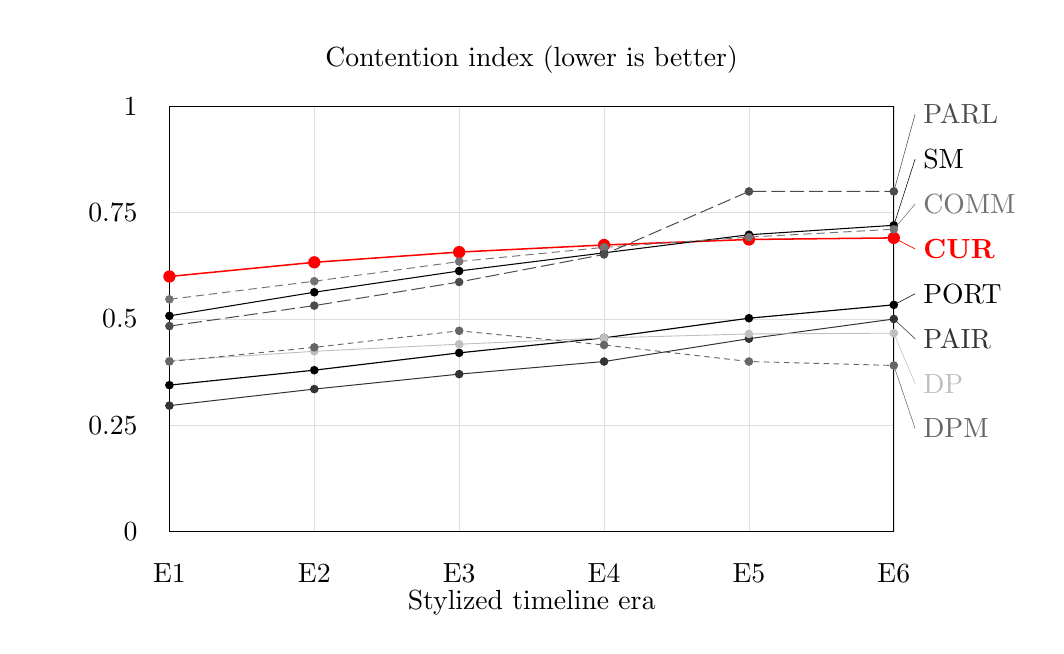
\begin{tikzpicture}[x=1mm,y=1mm]
\path[use as bounding box] (0,0) rectangle (128.0,76.0);
\draw[black!13,line width=0.18pt] (18.0,12.0) -- (110.0,12.0);
\node[anchor=east] at (15.2,12.0) {0};
\draw[black!13,line width=0.18pt] (18.0,25.5) -- (110.0,25.5);
\node[anchor=east] at (15.2,25.5) {0.25};
\draw[black!13,line width=0.18pt] (18.0,39.0) -- (110.0,39.0);
\node[anchor=east] at (15.2,39.0) {0.5};
\draw[black!13,line width=0.18pt] (18.0,52.5) -- (110.0,52.5);
\node[anchor=east] at (15.2,52.5) {0.75};
\draw[black!13,line width=0.18pt] (18.0,66.0) -- (110.0,66.0);
\node[anchor=east] at (15.2,66.0) {1};
\draw[black!12,line width=0.18pt] (18.0,12.0) -- (18.0,66.0);
\node[anchor=north] at (18.0,9.2) {E1};
\draw[black!12,line width=0.18pt] (36.4,12.0) -- (36.4,66.0);
\node[anchor=north] at (36.4,9.2) {E2};
\draw[black!12,line width=0.18pt] (54.8,12.0) -- (54.8,66.0);
\node[anchor=north] at (54.8,9.2) {E3};
\draw[black!12,line width=0.18pt] (73.2,12.0) -- (73.2,66.0);
\node[anchor=north] at (73.2,9.2) {E4};
\draw[black!12,line width=0.18pt] (91.6,12.0) -- (91.6,66.0);
\node[anchor=north] at (91.6,9.2) {E5};
\draw[black!12,line width=0.18pt] (110.0,12.0) -- (110.0,66.0);
\node[anchor=north] at (110.0,9.2) {E6};
\draw[black,line width=0.28pt] (18.0,12.0) rectangle (110.0,66.0);
\draw[red,line width=0.55pt] (18.0,44.4) -- (36.4,46.2) -- (54.8,47.5) -- (73.2,48.4) -- (91.6,49.1) -- (110.0,49.3);
\fill[red] (18.0,44.4) circle[radius=0.78];
\fill[red] (36.4,46.2) circle[radius=0.78];
\fill[red] (54.8,47.5) circle[radius=0.78];
\fill[red] (73.2,48.4) circle[radius=0.78];
\fill[red] (91.6,49.1) circle[radius=0.78];
\fill[red] (110.0,49.3) circle[radius=0.78];
\draw[black,line width=0.38pt] (18.0,39.4) -- (36.4,42.4) -- (54.8,45.1) -- (73.2,47.4) -- (91.6,49.7) -- (110.0,50.9);
\fill[black] (18.0,39.4) circle[radius=0.55];
\fill[black] (36.4,42.4) circle[radius=0.55];
\fill[black] (54.8,45.1) circle[radius=0.55];
\fill[black] (73.2,47.4) circle[radius=0.55];
\fill[black] (91.6,49.7) circle[radius=0.55];
\fill[black] (110.0,50.9) circle[radius=0.55];
\draw[black!55,line width=0.34pt,dash pattern=on 3pt off 1.8pt] (18.0,41.5) -- (36.4,43.8) -- (54.8,46.3) -- (73.2,48.1) -- (91.6,49.4) -- (110.0,50.4);
\fill[black!55] (18.0,41.5) circle[radius=0.55];
\fill[black!55] (36.4,43.8) circle[radius=0.55];
\fill[black!55] (54.8,46.3) circle[radius=0.55];
\fill[black!55] (73.2,48.1) circle[radius=0.55];
\fill[black!55] (91.6,49.4) circle[radius=0.55];
\fill[black!55] (110.0,50.4) circle[radius=0.55];
\draw[black!70,line width=0.36pt,dash pattern=on 5pt off 1.8pt] (18.0,38.1) -- (36.4,40.7) -- (54.8,43.7) -- (73.2,47.2) -- (91.6,55.2) -- (110.0,55.2);
\fill[black!70] (18.0,38.1) circle[radius=0.55];
\fill[black!70] (36.4,40.7) circle[radius=0.55];
\fill[black!70] (54.8,43.7) circle[radius=0.55];
\fill[black!70] (73.2,47.2) circle[radius=0.55];
\fill[black!70] (91.6,55.2) circle[radius=0.55];
\fill[black!70] (110.0,55.2) circle[radius=0.55];
\draw[black!80,line width=0.36pt] (18.0,28.0) -- (36.4,30.1) -- (54.8,32.0) -- (73.2,33.6) -- (91.6,36.5) -- (110.0,39.0);
\fill[black!80] (18.0,28.0) circle[radius=0.55];
\fill[black!80] (36.4,30.1) circle[radius=0.55];
\fill[black!80] (54.8,32.0) circle[radius=0.55];
\fill[black!80] (73.2,33.6) circle[radius=0.55];
\fill[black!80] (91.6,36.5) circle[radius=0.55];
\fill[black!80] (110.0,39.0) circle[radius=0.55];
\draw[black,line width=0.42pt] (18.0,30.6) -- (36.4,32.5) -- (54.8,34.7) -- (73.2,36.6) -- (91.6,39.1) -- (110.0,40.8);
\fill[black] (18.0,30.6) circle[radius=0.55];
\fill[black] (36.4,32.5) circle[radius=0.55];
\fill[black] (54.8,34.7) circle[radius=0.55];
\fill[black] (73.2,36.6) circle[radius=0.55];
\fill[black] (91.6,39.1) circle[radius=0.55];
\fill[black] (110.0,40.8) circle[radius=0.55];
\draw[black!25,line width=0.32pt] (18.0,33.7) -- (36.4,34.9) -- (54.8,35.8) -- (73.2,36.6) -- (91.6,37.1) -- (110.0,37.2);
\fill[black!25] (18.0,33.7) circle[radius=0.55];
\fill[black!25] (36.4,34.9) circle[radius=0.55];
\fill[black!25] (54.8,35.8) circle[radius=0.55];
\fill[black!25] (73.2,36.6) circle[radius=0.55];
\fill[black!25] (91.6,37.1) circle[radius=0.55];
\fill[black!25] (110.0,37.2) circle[radius=0.55];
\draw[black!60,line width=0.34pt,dash pattern=on 2pt off 1.6pt] (18.0,33.6) -- (36.4,35.4) -- (54.8,37.5) -- (73.2,35.7) -- (91.6,33.6) -- (110.0,33.1);
\fill[black!60] (18.0,33.6) circle[radius=0.55];
\fill[black!60] (36.4,35.4) circle[radius=0.55];
\fill[black!60] (54.8,37.5) circle[radius=0.55];
\fill[black!60] (73.2,35.7) circle[radius=0.55];
\fill[black!60] (91.6,33.6) circle[radius=0.55];
\fill[black!60] (110.0,33.1) circle[radius=0.55];
\draw[black!60,line width=0.2pt] (110.0,33.1) -- (112.7,25.1);
% legend-label label=DPM x=113.5 y=25.1
\node[anchor=west,inner sep=0.5pt,text=black!60] at (113.5,25.1) {DPM};
\draw[black!25,line width=0.2pt] (110.0,37.2) -- (112.7,30.8);
% legend-label label=DP x=113.5 y=30.8
\node[anchor=west,inner sep=0.5pt,text=black!25] at (113.5,30.8) {DP};
\draw[black!80,line width=0.2pt] (110.0,39.0) -- (112.7,36.5);
% legend-label label=PAIR x=113.5 y=36.5
\node[anchor=west,inner sep=0.5pt,text=black!80] at (113.5,36.5) {PAIR};
\draw[black,line width=0.2pt] (110.0,40.8) -- (112.7,42.2);
% legend-label label=PORT x=113.5 y=42.2
\node[anchor=west,inner sep=0.5pt,text=black] at (113.5,42.2) {PORT};
\draw[red,line width=0.25pt] (110.0,49.3) -- (112.7,47.9);
% legend-label label=CUR x=113.5 y=47.9
\node[anchor=west,inner sep=0.5pt,text=red] at (113.5,47.9) {\textbf{CUR}};
\draw[black!55,line width=0.2pt] (110.0,50.4) -- (112.7,53.6);
% legend-label label=COMM x=113.5 y=53.6
\node[anchor=west,inner sep=0.5pt,text=black!55] at (113.5,53.6) {COMM};
\draw[black,line width=0.2pt] (110.0,50.9) -- (112.7,59.3);
% legend-label label=SM x=113.5 y=59.3
\node[anchor=west,inner sep=0.5pt,text=black] at (113.5,59.3) {SM};
\draw[black!70,line width=0.2pt] (110.0,55.2) -- (112.7,65.0);
% legend-label label=PARL x=113.5 y=65.0
\node[anchor=west,inner sep=0.5pt,text=black!70] at (113.5,65.0) {PARL};
\node at (64.0,3.0) {Stylized timeline era};
\node[anchor=south] at (64.0,69.0) {Contention index (lower is better)};
\end{tikzpicture}
\endgroup
}
  \caption{Appendix rising-contention stress paths from the main comparison campaign. The index is \(0.50\cdot\)gridlock \(+0.30\cdot(1-\)revision moderation\()+0.20\cdot\)low-public-support enactment. Lower is better.}
  \label{fig:appendix-timeline-contention}
  \Description{Line chart of selected contention paths over six stylized eras.}
\end{figure}

\section{Chamber-Structure Supplement}

The chamber-structure campaign tests representation architecture, committee power, eligibility filters, and ex ante review separately from the main mechanism comparison.

% Auto-generated by scripts/reporting/summarize_chamber_structure.py
\begin{table}
  \caption{Chamber, apportionment, committee, and review family champions from the chamber-structure supplement. Values are averaged across the chamber campaign cases.}
  \label{tab:chamber-family-champions}
  \Description{Compact table of chamber-family champion scenarios and core metrics.}
  \scriptsize
  \begin{tabular}{llrrrr}
    \toprule
    Label & Family champion & Prod. & Comp. & Risk & Malapp. \\
    \midrule
    BICAM & Bicameral conflict & 0.31 & 0.27 & 0.86 & 0.00 \\
    ASSIGN & Committee assignment & 0.22 & 0.29 & 0.89 & 0.00 \\
    COMMP & Committee power & 0.25 & 0.28 & 0.87 & 0.00 \\
    CONV & Conventional benchmark & 0.34 & 0.25 & 0.85 & 0.00 \\
    REVIEW & Independent review & 0.34 & 0.25 & 0.85 & 0.00 \\
    ROUTE & Origination and routing & 0.31 & 0.27 & 0.86 & 0.00 \\
    OTHER & Other chamber design & 0.31 & 0.26 & 0.86 & 0.00 \\
    SEAT & Seat allocation & 0.34 & 0.25 & 0.85 & 0.00 \\
    SELECT & Selection and retention & 0.36 & 0.24 & 0.84 & 0.00 \\
    UPPER & Upper-chamber composition & 0.36 & 0.26 & 0.84 & 0.12 \\
    \bottomrule
  \end{tabular}
\end{table}


\begin{figure}
  \centering
  % Auto-generated by scripts/reporting/summarize_chamber_structure.py
\begingroup
\setlength{\unitlength}{1mm}
\begin{picture}(128,84)
\scriptsize
\put(22.0,14.0){\color{black!15}\line(0,1){58.0}}
\put(22.0,14.0){\color{black!15}\line(1,0){95.0}}
\put(22.0,11.0){\makebox(0,0){0}}
\put(18.0,14.0){\makebox(0,0)[r]{0}}
\put(45.8,14.0){\color{black!15}\line(0,1){58.0}}
\put(22.0,28.5){\color{black!15}\line(1,0){95.0}}
\put(45.8,11.0){\makebox(0,0){0.25}}
\put(18.0,28.5){\makebox(0,0)[r]{0.25}}
\put(69.5,14.0){\color{black!15}\line(0,1){58.0}}
\put(22.0,43.0){\color{black!15}\line(1,0){95.0}}
\put(69.5,11.0){\makebox(0,0){0.5}}
\put(18.0,43.0){\makebox(0,0)[r]{0.5}}
\put(93.2,14.0){\color{black!15}\line(0,1){58.0}}
\put(22.0,57.5){\color{black!15}\line(1,0){95.0}}
\put(93.2,11.0){\makebox(0,0){0.75}}
\put(18.0,57.5){\makebox(0,0)[r]{0.75}}
\put(117.0,14.0){\color{black!15}\line(0,1){58.0}}
\put(22.0,72.0){\color{black!15}\line(1,0){95.0}}
\put(117.0,11.0){\makebox(0,0){1}}
\put(18.0,72.0){\makebox(0,0)[r]{1}}
\put(22.0,14.0){\line(1,0){95.0}}
\put(22.0,14.0){\line(0,1){58.0}}
\put(51.5,29.6){\makebox(0,0){\color{black!45}\rule{1.6mm}{1.6mm}}}
\linethickness{0.10mm}
{\color{black!50}\qbezier[6](51.5,29.6)(53.5,26.4)(55.5,23.2)}
\linethickness{0.25mm}
% point-label label=BICAM pointX=51.5 pointY=29.6 labelX=55.5 labelY=23.2 anchor=l leader=1
\put(55.5,23.2){\makebox(0,0)[l]{\color{black!45}BICAM}}
\put(43.2,30.7){\makebox(0,0){\color{black!45}\rule{1.6mm}{1.6mm}}}
\linethickness{0.10mm}
{\color{black!50}\qbezier[6](43.2,30.7)(41.2,33.9)(39.2,37.1)}
\linethickness{0.25mm}
% point-label label=ASSIGN pointX=43.2 pointY=30.7 labelX=39.2 labelY=37.1 anchor=r leader=1
\put(39.2,37.1){\makebox(0,0)[r]{\color{black!45}ASSIGN}}
\put(45.5,30.0){\makebox(0,0){\color{black!45}\rule{1.6mm}{1.6mm}}}
\linethickness{0.10mm}
{\color{black!50}\qbezier[6](45.5,30.0)(47.5,33.2)(49.5,36.4)}
\linethickness{0.25mm}
% point-label label=COMMP pointX=45.5 pointY=30.0 labelX=49.5 labelY=36.4 anchor=l leader=1
\put(49.5,36.4){\makebox(0,0)[l]{\color{black!45}COMMP}}
\put(53.9,28.4){\makebox(0,0){\color{red}\rule{2.0mm}{2.0mm}}}
\linethickness{0.10mm}
{\color{red!55}\qbezier[6](53.9,28.4)(57.5,28.9)(61.1,29.3)}
\linethickness{0.25mm}
% point-label label=CONV pointX=53.9 pointY=28.4 labelX=61.1 labelY=29.3 anchor=l leader=1
\put(61.1,29.3){\makebox(0,0)[l]{\color{red}CONV}}
\put(53.9,28.4){\makebox(0,0){\color{black!45}\rule{1.6mm}{1.6mm}}}
\linethickness{0.10mm}
{\color{black!50}\qbezier[6](53.9,28.4)(60.3,26.2)(66.7,24.0)}
\linethickness{0.25mm}
% point-label label=REVIEW pointX=53.9 pointY=28.4 labelX=66.7 labelY=24.0 anchor=l leader=1
\put(66.7,24.0){\makebox(0,0)[l]{\color{black!45}REVIEW}}
\put(51.7,29.5){\makebox(0,0){\color{black!45}\rule{1.6mm}{1.6mm}}}
\linethickness{0.10mm}
{\color{black!50}\qbezier[6](51.7,29.5)(49.7,26.3)(47.7,23.1)}
\linethickness{0.25mm}
% point-label label=ROUTE pointX=51.7 pointY=29.5 labelX=47.7 labelY=23.1 anchor=r leader=1
\put(47.7,23.1){\makebox(0,0)[r]{\color{black!45}ROUTE}}
\put(51.2,29.3){\makebox(0,0){\color{black!45}\rule{1.6mm}{1.6mm}}}
\linethickness{0.10mm}
{\color{black!50}\qbezier[6](51.2,29.3)(49.2,32.5)(47.2,35.7)}
\linethickness{0.25mm}
% point-label label=OTHER pointX=51.2 pointY=29.3 labelX=47.2 labelY=35.7 anchor=r leader=1
\put(47.2,35.7){\makebox(0,0)[r]{\color{black!45}OTHER}}
\put(53.9,28.4){\makebox(0,0){\color{black!45}\rule{1.6mm}{1.6mm}}}
\linethickness{0.10mm}
{\color{black!50}\qbezier[6](53.9,28.4)(55.9,31.6)(57.9,34.8)}
\linethickness{0.25mm}
% point-label label=SEAT pointX=53.9 pointY=28.4 labelX=57.9 labelY=34.8 anchor=l leader=1
\put(57.9,34.8){\makebox(0,0)[l]{\color{black!45}SEAT}}
\put(56.0,28.0){\makebox(0,0){\color{black!45}\rule{1.6mm}{1.6mm}}}
\linethickness{0.10mm}
{\color{black!50}\qbezier[6](56.0,28.0)(56.0,23.0)(56.0,18.0)}
\linethickness{0.25mm}
% point-label label=SELECT pointX=56.0 pointY=28.0 labelX=56.0 labelY=18.0 anchor=c leader=1
\put(56.0,18.0){\makebox(0,0)[c]{\color{black!45}SELECT}}
\put(55.9,29.1){\makebox(0,0){\color{black!50}\rule{1.6mm}{1.6mm}}}
\linethickness{0.10mm}
{\color{black!50}\qbezier[6](55.9,29.1)(62.3,31.3)(68.7,33.5)}
\linethickness{0.25mm}
% point-label label=UPPER pointX=55.9 pointY=29.1 labelX=68.7 labelY=33.5 anchor=l leader=1
\put(68.7,33.5){\makebox(0,0)[l]{\color{black!50}UPPER}}
\put(69.5,4.0){\makebox(0,0){Productivity $\uparrow$}}
\put(7.0,43.0){\rotatebox{90}{Compromise $\uparrow$}}
\put(99.0,76.0){\makebox(0,0)[l]{darker = more malapportioned}}
\end{picture}
\endgroup

  \caption{Chamber-structure family champions from the supplemental chamber campaign, zoomed to the observed champion range so clustered family labels remain readable. The axes keep the paper's central productivity/revision-moderation comparison visible; malapportionment remains in Table~\ref{tab:chamber-family-champions} because the champion set has little variation on that metric.}
  \label{fig:chamber-productivity-compromise}
  \Description{Scatter plot of chamber family champion productivity and revision moderation, with the conventional benchmark marked by a distinct label and marker.}
\end{figure}

\section{Assumptions and Limitations}
\label{sec:appendix-limitations}

The policy space is one-dimensional. Public benefit is generated rather than empirically estimated. Legislators are synthetic and do not represent named real officials. Lobby groups are abstract collective actors. The empirical flow layer screens plausible ranges but does not fit raw datasets automatically. Leadership, initiative, conference, judicial, court-architecture, district-public, influence-system, long-horizon learning, and norm-erosion processes are stylized mechanism prototypes rather than detailed institutional models. Institutional mechanisms are simplified so they can be compared in bundles without modeling the full legal, administrative, judicial, media, and electoral environment. Omnibus and package bargaining are proxies for side payments, delays, exemptions, jurisdictional trades, distributive load, and harm reduction, not full models of legal text, appropriations, or multidimensional coalition formation.

\section{Reproducibility}
\label{sec:appendix-reproducibility}

The main reproducibility entrypoints are:

\begin{itemize}
  \item \texttt{make test}: compile and run the simulator test suite.
  \item \texttt{make campaign} or \texttt{make paper-campaign}: regenerate the comparison campaign.
  \item \texttt{make calibrate}: run empirical flow benchmark screening.
  \item \texttt{make seed-robustness-check}: run multi-seed checks for paper scenarios.
  \item \texttt{make validation-readiness}: check optional raw-input shape.
  \item \texttt{make empirical-validation}: summarize any present raw inputs.
  \item \texttt{make empirical-bridge}: map raw summaries to simulator proxies for empirical flow smoke tests.
  \item \texttt{make validation-gap-report}: generate the paper-facing empirical-boundary report. Adapter fixtures live separately and do not count as raw empirical data.
  \item \texttt{make build-bill-progression-raw}: rebuild the documented Congress.gov bill-progression raw sample when a Congress.gov API key is available.
  \item \texttt{make build-core-raw-validation}: rebuild the broader Voteview, Congress.gov-derived, and Senate LDA empirical comparison samples when network access and any required API key are available.
  \item \texttt{make ablation-analysis}, \texttt{make manipulation-stress}, and \texttt{make mechanism-diagnostics}: run mechanism ablations, manipulation stress tests, and the generated diagnostics table workflow.
  \item \texttt{make family-screen}, \texttt{make catalog-breadth}, and \texttt{make chamber-structure}: run breadth-catalog and chamber-structure diagnostics.
  \item \texttt{make paper}: build the paper and appendix PDFs.
  \item \texttt{make reproduce-paper-offline}: run the no-network paper reproduction path from fixed seeds and local summaries.
  \item \texttt{make supplement-anonymous}: build the double-blind supplement package.
  \item \texttt{make public-provenance}: after review, generate a non-anonymous provenance manifest.
\end{itemize}

The review package includes generated campaign reports and PDFs. Public repository identifying details are withheld during double-blind review and can be restored after review if permitted.

\section*{Use of Large Language Model Tools}

The research question and core simulator idea originated with the human author. OpenAI ChatGPT/Codex tools available in the authoring environment during the April--May 2026 revision period were used for grammar and style editing, restructuring suggestions, code debugging assistance, and drafting assistance for portions of the simulator implementation, generated-report scripts, and manuscript prose. LLM tools were not used as authors. Tool outputs were edited and checked by the author; references, code outputs, experiments, tables, figures, and claims were manually reviewed against the repository artifacts before inclusion. No large language model is listed as an author.

\bibliographystyle{ACM-Reference-Format}
\bibliography{references}

\end{document}
